\chapter{Caratterizzazione di Dati Misurati}
Resi noti una serie di dati misurati, quello che si vuole andare a fare è trovare un modello statistico che mi permetta di avere un'approssimazione valida di tali dati. Ci sono varie tipologie di tecniche e di approcci. Per grandi quantità di dati si farà un utilizzo massiccio della \textbf{Statistica inferenziale}, che comprende tutta una serie di metodi che permettono di andare a stimare un modello quantò più opportuno possibile ai dati che si stanno andando ad analizzare

\subsection{Media, Mediana e Moda}
Dato un insieme di dati, si possono andare a valutare 3 valori principali (e scalari), che ci permettono di approssimare (in maniera grossolana), la nostra distribuzione di dati (rappresentabile, anche, mediante un istogrammma). I valori a cui si fa riferimento sono:
\begin{itemize}
    \item \textbf{Media}: Media statistica di tutti i valori che si sta andando a considerare. Se si ha un set di valoi \(X = (x_1,x_2,\dots,x_n)\), allora definiamo come media:
    \[
    \overline{X} = \frac{1}{n}\sum_{i=1}^{n}x_i
    \]
    La media, però, non tiene conto dell'asimmetria dei dati (skewness), quindi se ad esempio un sistema ha dei tempi di ripsosta sempre stabili, e poi, un singolo caso di tempo di risposta lungo, potrebbe avere la stessa media di un sistema che ha mediamente tempi di risposta più lunghi (molto sensibile ad eventuali comportamenti limite)
    \item \textbf{Mediana}: La mediana di un set di valori \(X = (x_1,x_2,\dots,x_n)\) è data dalla selezione del valore centrale del set di valori ordinati. Per capire, si ordina il set di valori \(X\) e poi si seleziona l'elemento presente in \(\left\lfloor\frac{n}{2}\right\rfloor\). Ciò però presenta un problema, se il numrero di valori è dispari allora io seleziono l'unica posizione centrale presente (es. Se ho 3 elementi seleziono 1), mentre se ho un valore pari devo trovare un modo con cui scegliere quale elemento considerare, pertanto, essendo due i valori centrali, se ne fa la media (es. se ho 4 elementi, farò la media del valore in posizione 1 ed in posizione 2). La mediana a differenza della media viene presa direttamente dai valori reali e non calcolata considerando tutti i valori, ciò gli permette di essere più resistente agli outlier e sopratutto a distribuzioni asimettriche (resistente alla skewness)
    
    \item \textbf{Moda}: La moda rappresenta il valore più probabile all'interno di una distribuzione (quello presentato più volte). Di conseguenza tiene conto del picco presente nell'istrogramma. Il problema della moda è che può non esistere (caso di distribuzioni uniformi), oppure può assumere più di un valore (immaginare una distribuzione bi-gaussiana). Nonostante le considerazioni precedenti, la media è totalmente immune agli outlier (vedo solo il più probabile), e mi permette di evitare anche le ambiguità di una particolare distribuzione
\end{itemize}

\begin{info}
Nella descrizione dei parametri precedenti si è parlato di asimettrie dei dati (skewness dei dati), tale valore per piccole quantità di campioni può essere approssimato con la formula:
\[
skewness = \frac{y_{max}}{y_{min}}
\]
Da tale formula comprendo che più il valore è alto e più i dati sono "asimettrici". Ma tale considerazione è più corretta quanto più è piccola la quantità di campioni che sto andando a considerare 
\end{info}


Un semplice criterio per decidere quale tipologia di metrica utilizzare è quella mostrata in figura [\ref{img:criterio-media-mediana}]

\begin{figure}[h]
\centering
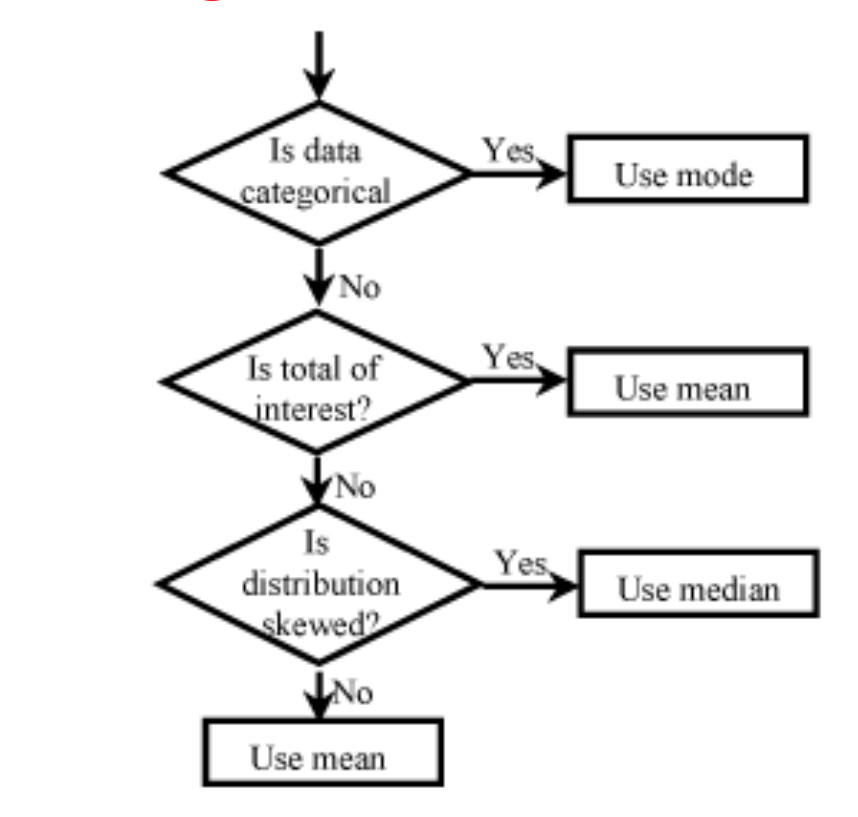
\includegraphics[width=.5\textwidth]{img/chapter-4/criterio-media-mediana.png}
\caption{Semplice schema di un criterio per la scelta della metrica da utilizzare}\label{img:criterio-media-mediana}
\end{figure}

I valori descritti, oltretutto, possono essere ottenuti osservando anche la distribuzione dei dati mediante degli istogrammi di occorrenza. In questo modo è anche più facile campire quale metrica sia meglio utilizzare.

\begin{figure}[H]
\centering
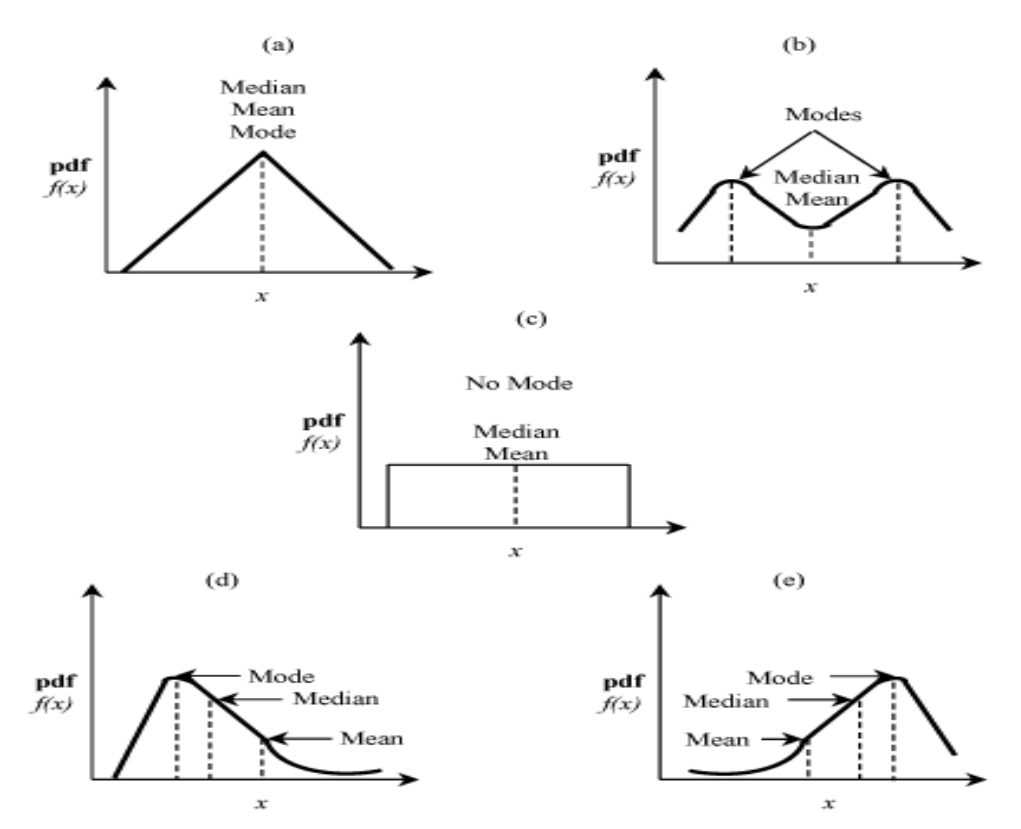
\includegraphics[width=.5\textwidth]{img/chapter-4/grafici-media-mediana.png}
\caption{Grafici illustrativi dei parametri discussi}\label{img:grafici-media-mediana}
\end{figure}

\subsection{Indici di dispersione}
Andare ad approssimare una distribuzione di valori con un singolo valore non basta, tale informazione non mi permette di considerare anche la \textbf{variabilità} che i dati possono avere nel tempo.
Uno strumento utile per avere un'idea della variabilità, sono gli \textbf{indici di dispersione}. Tra le metriche più utilizzate possiamo trovare:
\begin{itemize}
\item \textbf{Range}: Il range è un parametro molto basilare che viene calcolato come: \(v_{max} - V{min}\). Tale metrica, per quanto semplice, è anche molto poco resistente agli outlier
\item \textbf{Varianza campionaria (o deviazione standard)}: Tale parametro è strettamente calcolato dai dait e dipende dalla loro distribuzione
\item \textbf{10- e -90 Percentile}: Prendendo una distribuzione di dati si vanno a considerare due valori:
\begin{itemize}
    \item \textbf{\(P10\)}: Valore dei dati sotto il quale cade il 10\% dei dati considerati
    \item \textbf{\(P90\)}: Valore dei dati sotto il quale cade il 90\% dei dati considerati (quindi solo il restante 10\% è maggiore)
\end{itemize}
Si definisce poi come indice di dispersione il range calcolato su tali valori: \(range = P90-P10\). Se vediamo tali valori in riferimento alla pdf dei dati (il loro istogramma) e alla CDF. Si ha che per calcolare il valore P90 e P10, vado a valutare il valore della CDF in base al percentile ricercato (\(F(x_p) = 0.10\) o \(0.90\)), oppure, nel caso della pdf vado a calutare l'integrale (guardare la relazione tra CDF e pdf)\(\left [\int_{-\infty}^{x_p}f(x)dx = 0.10 | 0.90\right ]\). Il percentile solitamente può essere chiamato anche \textbf{quartile}. La differenza sta nella notazione, per il quartile si dice \(0.1\)-quartile (\(\alpha\)-quartile), mentre il percentile si esprime come 10-percentile (\(100*\alpha\)-percentile). Per stimare tali valori su un insieme di dati discreto (quindi non distribuzioni continue su cui effettuare integrali o derivate), posso andare ad effettuare, prima un ordinamento e poi a selezionare uno specifico valore in base alla \(\alpha\) scelta. Precisamente si va a selezionare il valore in posizione: \([(n-1)*\alpha + 1]\)

\item \textbf{Semi Inter-Quartile Range}: Tale metrica va ad utilizzare la definizione di due particolari casi di quartile. Più precisamente si va a considerare i quartili: \(0.75\)-quartile (75-percentile) [o terzo quartile] ed il \(0.25\)-quartile (25-percentile) [o primo quartile]. Tali valori sono poi combinati e si va a calcolare il valore del Semi Inter-Quartile Range come:
\[
SIQR = \frac{Q_3 - Q_1}{2}
\]

\item \textbf{Mean Absolute Deviation}: Vado a considerare la somma delle deviazioni, ma che sia sottoposta prima all'operazione di modulo, in modo da evitale l'azzeramento della somma delle deviazioni (come visto nel capitolo precedente). La formula è la seguente:
\[
MAD = \frac{1}{n}\sum_{i=1}^{n}|x_i - \overline{x}|
\]
Dove \(\overline{x}\) è la media dei valori: \(x_1,x_2, \dots, x_n\).

\end{itemize}

Un elemento utile quando si sta guardando il grafico dei dati è il \textbf{boxplot}. Il boxplot ci da un informazione grafica iniziale su dove i valori di interesse per il calcolo delle diverse metriche si trovino. Principalmente ci permette di poter osservare le seguenti metriche [\ref{img:boxplot}]:
\begin{itemize}
    \item \textbf{Valore massimo}
    \item \textbf{Valore minimo}
    \item \textbf{Mediana}(o 0.5-quartile/secondo quartile)
    \item \textbf{Primo Quartile}(0.25-quartile)
    \item \textbf{Terzo Quartile}(0.75-quartile)
    \item \textbf{Semi Inter-Quartile Range}
\end{itemize}

\begin{figure}[H]
\centering
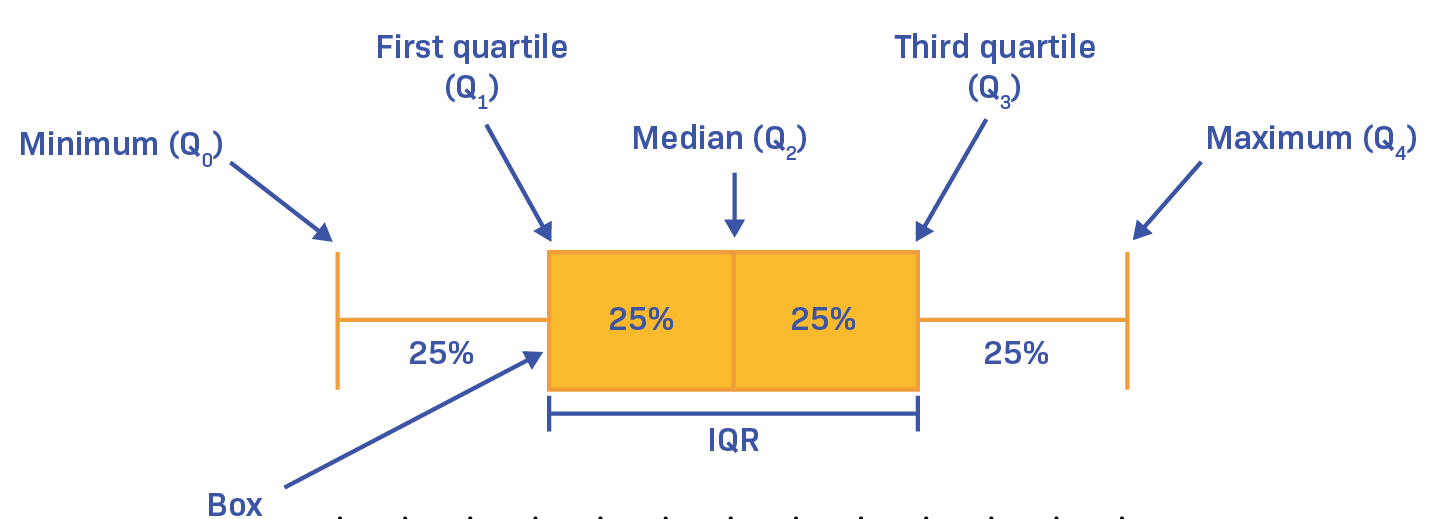
\includegraphics[width=.7\textwidth]{img/chapter-4/boxplot.png}
\caption{Struttura di un boxplot}\label{img:boxplot}
\end{figure}

La stima dell'indice di dispersione è qualcosa di complicato, sopratutto quando ci sono in mezzo gli outlier. Pertanto, solitamente, come metrica al posto della varianza (che non è completamente immune agli outlier), si preferisce utilizzare il Semi Iter-Quartile Range (SIRQ), che è più resistente alla presenza di outlier (anche più di qualcuno). Mentre come metrica centrale si preferisce l'uso della mediana, questo poichè ci è assicurato che esista (a differenza della moda), e sopratutto che faccia parte dell'insieme di valori considerato (diversamente dalla media). Questo spiega anche la costruzione del boxplot e dei valori che va a mettere in evidenza.

\subsection{Quantile-Quantile Plot}
Il \textbf{Quantile-Quantile Plot} è un metodo che ci permette di confrontare se due popolazioni hanno una distribuzione simile o meno. Nel nostro caso lo si utilizzerà per confrontare la distribuzione della nostra popolazione rispetto alla distribuzione normale.
La composizione di base di un grafico quantile-quantile generico è la seguente:
Si va a definire un punto \(p\) come \(p = (x_i, y_i)\), dove \(x_i\) è il valore teorico dell' i-esimo quantile, mentre \(y_i\) è il valore reale dell'i-esimo quantile. Per quanto riguarda i parametri reali non è complicato trovare i quartili (basta utilizzare la specifica formula in base ad \(\alpha\)), mentre per i parametri teorici risulta più complesso dato che bisogna trovare il modo di invertire la CDF. Per ricavare i valori della normale (funzione gaussiana di media nulla e varianza unitaria). Vado a calcolare il quartile come: \(q_i = \frac{i-0.5}{2}\), da cui posso ricavare il valore teorico come: \(x_i = 4.91\left [ q_i^{0.14} - (1-q_i)^{0.14} \right ]\).
Quindi, in generale, data una popolazione posso plottare il grafico utilizzando le metriche esposte in precedenza, e confrontare la distribuzione dei dati reali con quelli di una normale. In questo modo cerco di capire quanto la distribuzione della popolazione sia simile ad una distribuzione gaussiana. Alcuni esempi sono mostrati alla figura: [\ref{img:qqplot}]

\begin{figure}[h]

\centering
\begin{subfigure}[b]{0.5\textwidth}
\centering
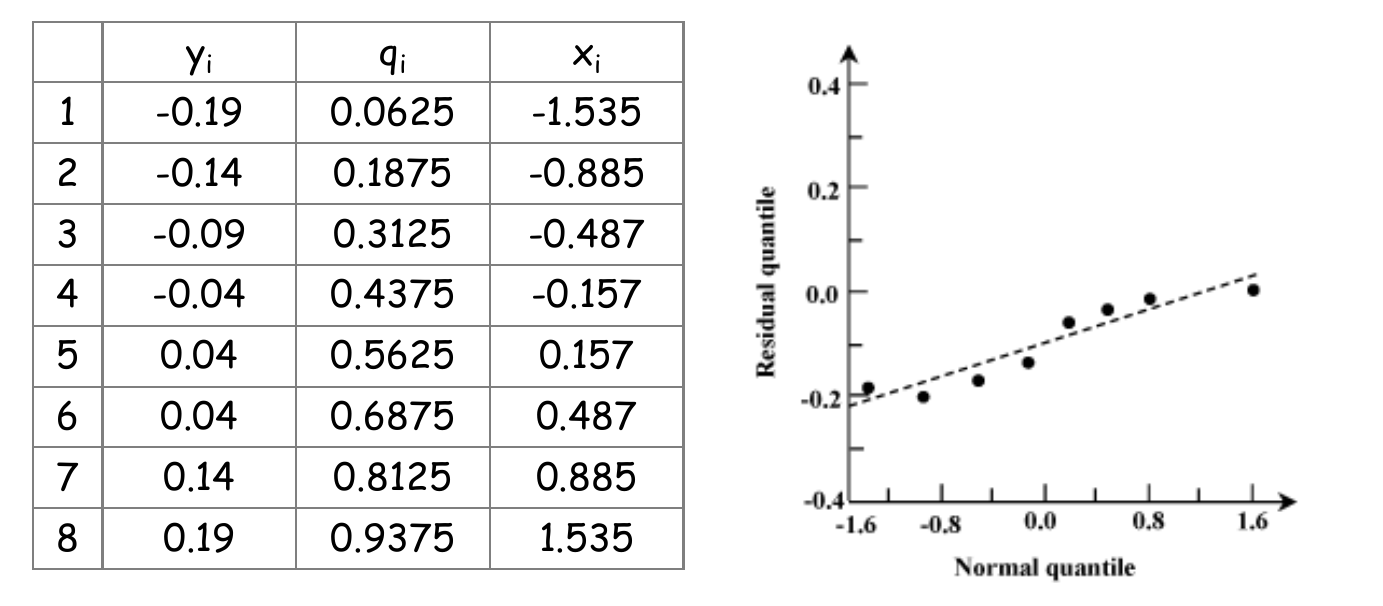
\includegraphics[width=\textwidth]{img/chapter-4/qqplot-ex.png}
\caption{Esempio di Quantile-Quantile plot rispetto alla normale}\label{img:qqplot-ex}
\end{subfigure}

\hfill

\begin{subfigure}[b]{0.6\textwidth}
\centering
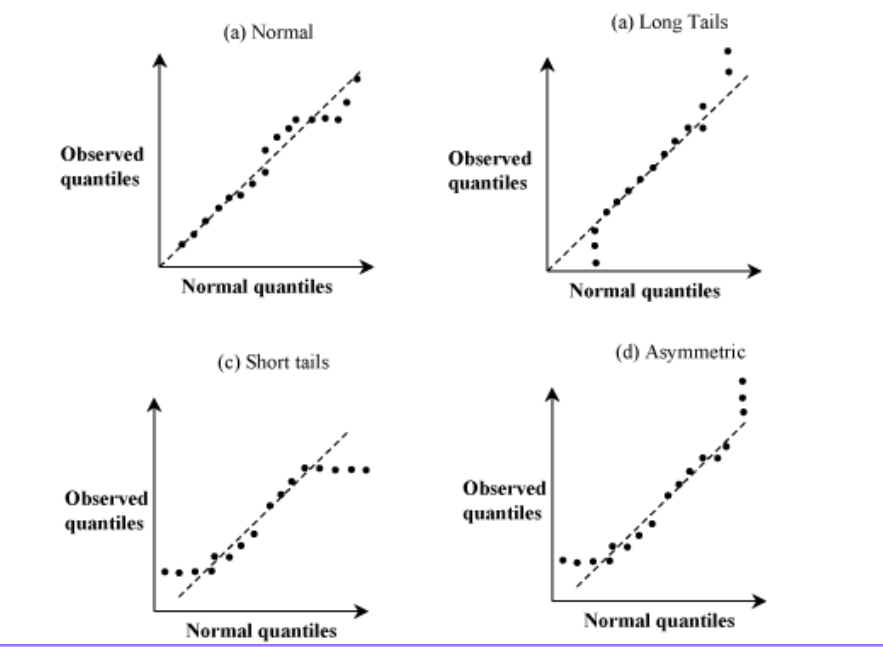
\includegraphics[width=\textwidth]{img/chapter-4/qqplot-confronto.png}
\caption{Diverse tipologie di rappresentazioni in base alla natura della popolazione}\label{img:qqplot-confronto}
\end{subfigure}

\caption{Applicazioni della Quanitile-Quantile plot (o  rappresentazione Quantile-Quantile)}\label{img:qqplot}
\end{figure}

\clearpage
\subsection{Intervalli di confidenza e dimensione del campionamento}
Solitamente, andare a considerare tutta la popolazione, potrebbe essere oneroso, pertanto, si potrebbe considerare di fare delle valutazioni su un numero minore di componenti estratte in maniera randomica (campionamento della popolazione). La problematica principale risiede nelle assunzioni che si potrebbe fare sulle statistiche della popolazione intera, ovvero, calcolare qualche valore per l'intera popolazione a partire dalla popolazione intera. Tali metodoligie sono sotto il nome di \textbf{statistica inferenziale}.
Per comprenderne bene il legame osservare l'immagine [\ref{img:statistica-inferenziale}].

\begin{figure}[h]
\centering
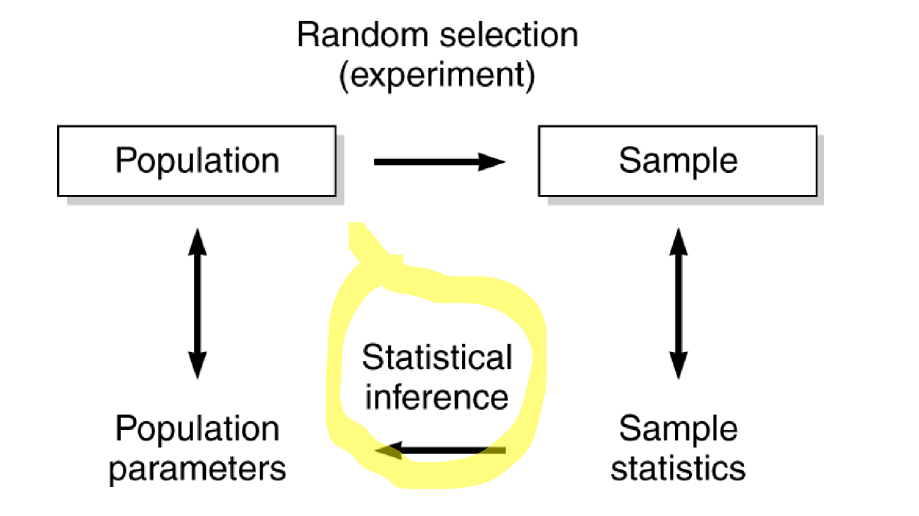
\includegraphics[width=.7\textwidth]{img/chapter-4/statistical-inference.png}
\caption{Collocazione logica della statistica inferenziale}\label{img:statistica-inferenziale}
\end{figure}

\subsubsection{Campioni e Popolazione}
\uppercase{è} importante definire cosa si intende quando si sta parlando di popolazione o di campioni, ciò ci permetterà di poter definire tutta una serie di principi statistici, utili, per effettuare l'inferenza statistica.
Formalmente si definisce \textbf{popolazione} l'insieme totale di tutte le componenti (o istanze), mentre si definisce \textbf{Campione}(O Sample), un insieme di n osservazioni provenienti dai campioni. In generale è importante, definire anche il significato di \textbf{parametri}, i dati associati alla popolazione, essi saranno indicati con le lettere greche (ad esempio la media e la varianza associate alla popolazione, tali valori per qualunque saranno i campioni estratti, non varieranno [saranno costanti]); mentre si definiscono \textbf{statistiche} i valori associati ai sample della popolazione, esse saranno rappresentate da lettere comuni (tali valori variano da campione a campione e quindi non sono costanti).

\begin{info}\label{inf:distribuzioni-Campionarie}
\textit{Tale pezzo non è richiesto ai fini dell'esame ma potrebbe essere utile in una fase di approfondimento e studio della statistica inferenziale}
    \\
\textbf{Distribuzioni Campionarie}\\
Si definisce \textbf{Distribuzione Campionaria}, una distribuzione di probabilità associata alla variabile aleatoria \(\overline{X}\), che è la composizione di diverse osservazioni \(X_1, X_2, \dots, X_n\) che sono ricavate da k-campioni della popolazione iniziale. \(\overline{X}\) non è altro che una variabile aleatoria associata alla media delle osservazioni (media campionaria).
\begin{warn}
Quando parliamo di \(\overline{X}\) stiamo parlando della variabile aleatoria (quindi un valore casuale), mentre la distribuzione campionaria è la funzione di distribuzione di probabilità(pdf) associata ad \(\overline{X}\)
\end{warn}

Pertanto, possiamo definire \(\overline{X}\) come:
\[
\overline{X} = \frac{X_1 + X_2 + \dots + X_n}{n}
\]
Da cui, applicando il \textbf{teorema fondamentale della media}, si ottiene che:
\[
E(\overline{X}) = \frac{E(X_1) + E(X_2) + \dots + E(X_n)}{n}
\]
Andando a considerare un caso più semplice, dove la popolazione ha media nota e pari a \(\mu\) e varianza \(\sigma^2\), e dove le variabili aleatorie \(X_1, X_2, \dots, X_n\), associate alle osservazioni dei campioni, sono delle variabili aleatorie indipendenti ed identicamente distribuite (sono la stessa variabile aleatoria con media \(\mu\) e varianza \(\sigma^2\), allora si può dire che:
\[
E(\overline{X} = \frac{\mu + \mu + \dots + \mu}{n} = \mu)
V(\overline{X}) = E((\overline{X} - \mu)^2) = \frac{\sigma^2 + \sigma^2 + \dots + \sigma^2}{n^2} = \frac{\sigma^2}{n} 
\]
Da tali formule si sono ricavati dei valori associati alla distribuzione campionaria, dette statistiche. Com'è possibile notare, più la dimensione del sample size cresce e più la varianza diminuisce, ciò ci fa capire che l'errore fatto sulla media diminuisce man mano (base per la valutazione dello standard error).
Andando ad invalidare le ipotesi fatte sulla struttura della popolazione (sulla sua distribuzione di probabilità), allora si può andare a valutare il \textbf{Teorema del limite centrale}.
\end{info}

\subsubsection{Standard Error}
Quando vado a valutare le statistiche riferite ai vari campioni presi dalla popolazione, con sample size pari ad n, voglio capire quanto queste siano effettivamente vicine a quelle reali. La problematica risiede proprio nel calcolo dei parametri. Di base, non si possono fare delle assunzioni sulla distribuzione di probabilità della popolazione (solitamente non è gaussiana, ma ha una forma generica o skewed (ambigua)). Pertanto non posso andare a valutare la varianza campionaria, questo poichè non posso fare assunzioni. Pertanto, in questi casi, ci viene in aiuto il \textbf{teorema del limite centrale}.
Il \textbf{teorema del limite centrale} ci dice che:
\\\textbf{Ipotesi}\\
Siano \(X_1, X_2, \dots, X_n\), n-variabili aleatorie Indipendenti ed identicamente distribuite (hanno tutte la stessa distribuzione, poichè la loro base dei dati è la stessa)
\\
Sia la sample size n, un valore orientativamente grande \(n>=30\)
\\
\textbf{Tesi}
\\
Allora posso dire che la \textbf{distribuzione campionaria} della media (distribuzione della variabile aleatori \(\overline{X}\)), è riconducibile ad una funzione normale con:
\begin{itemize}
    \item \textbf{Media} pari a \(\mu\) (media della popolazione)
    \item \textbf{Varianza} pari a \(\frac{\sigma^2}{n}\) (o deviazione standard \(\frac{\sigma}{\sqrt n}\))
\end{itemize}
Se la sample size è relativamente bassa (empiricamente minore di 30), la distribuzione ha un'andamento differente chiamato \textbf{t-student}. (Questo accade poichè, solitamente, non conoscendo la varianza reale della distribuzione globale, si potrebbe andare ad utilizzare la varianza campionaria, ma tale varianza avrà anche lei un margine di errore [è una variabile aleatoria a n-1 gradi di libertà]. Di conseguenza quella relazione diventa una relazione assimilabile alla t-student).

\begin{info}
\textit{Tale pezzo non è richieto per lo svolgimento dell'esame, ma solo al fine di approfondire alcuni concetti}
\\
Seguendo quello che si è visto nel precedente approfondimento [\ref{inf:distribuzioni-Campionarie}]; Il teorema del limite centrale non è altro che la conseguenza della composizione della variabile aleatoria \(\overline{X}\), rispetto alle variabili aleatorie associate ai campioni. Se le variabili aleatorie sono indipendenti (ce lo assicurano le indipendenze tra le varie osservazioni) ed identicamente distribuite (il fatto che le varie variabili abbiano la stessa pdf(e quindi non lo stesso valore), ci assicura, che la  media di tutte le distribuzioni sia \(\mu\)), allora il teorema del limite centrale non è altro che la dimostrazione del caso particolare che si è mostrato in precedenza. Se si vuole avere una maggior formalità nell'esporre il teorema del limite centrale si può andare a definire, una nuova variabile aleatoria \(Z\), come:
\[
Z = \frac{\overline{X} - \mu}{\sigma / \sqrt{n}} 
\xrightarrow{\,n \to \infty\,} 
\mathcal{N}(0,1)
\]
Tale Z, solitamente, viene assimilata ad una \textbf{t-student}, poichè non è sempre detto che si conosca la \(\sigma\) reale associata alla popolazione, pertanto si va ad utilizzare la varianza campionaria \(s\). Data questa "sostituzione", come per la media, anche per la varianza bisognerebbe andare a definire degli intervalli di confidenza e degli errori rispetto al valore reale (pertanto viene trattata come una variabile aleatoria chi-quadrata), ciò ci permette di dire che la variabile aleatoria sopracitata \(Z\), sia a tutti gli effetti una \textbf{t-student}.
\end{info}

Il \textbf{Teorema del limite centrale} non fa alcuna ipotesi sulla distribuzione della popolazione di partenza. Pertanto si mostra un esempio di applicazione mediante la figura [\ref{img:central-limit}]

\begin{figure}[h]
\centering
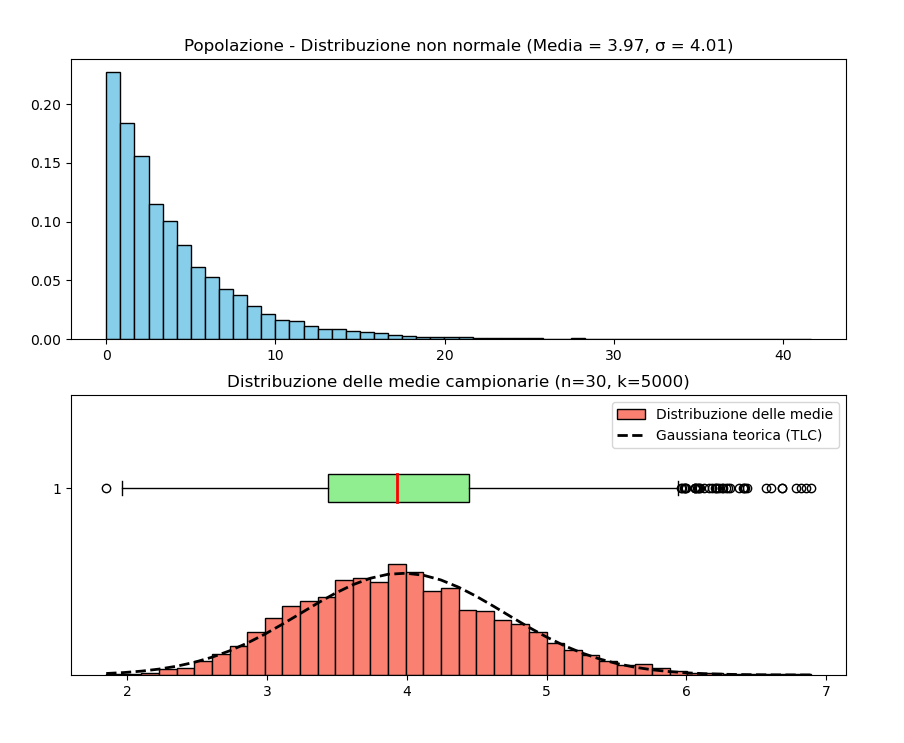
\includegraphics[width=.9\textwidth]{img/chapter-4/central-limit.png}
\caption{Applicazione del teorema del limite centrale}\label{img:central-limit}
\end{figure}

\subsubsection{Intervalli di confidenza}
Per comprendere appieno il significato di \textbf{intervallo di confidenza}, allora, bisogna esprimere in maniera migliore la variabile aleatoria \(\overline{X}\). Quello che si vuole andare a fare è normalizzarla, per cercare di ricondurre la distribuzione ad una normale con varianza unitaria. 
Formalmente potremo dire che:
\\
Siano \(X_1,X_2, \dots, X_n\) variabili aleatroie associate ai campioni di una popolazione che ha una distribuzione normale con una media non nota \(\mu\) ed una varianza nota \(\sigma^2\). Allora, la variabile aleatoria associata all'operazione di media \(\overline{X}\) è, teoricamente, normale, centrata in \(\mu\) e con varianza \(\sigma^2/n\). Pertanto, posso andare a normalizzare tale distribuzione di probabilità ad una normale standard mediante l'applicazione della seguente formula (simile allo z-score):
\[
Z = \frac{\overline{X} - \mu}{\sigma/\sqrt{n}}
\]

\begin{warn}
Per ora non si è ancora detto nulla sul come sia fatta la varianza, pertanto, se ci sono dei dubbi, risulta perfettamente in linea dato che ancora deve essere affrontata la valutazione della varianza
\end{warn}

Un \textbf{Intervallo di confidenza}, quindi, non è altro che un intervallo numerico in cui la media ricade. In maniera formale, un intervallo di confidenza viene rappresentato mediante l'intervallo \([l,u]\), che ha la seguente caratteristica: \(l\leq\mu\leq u\). \(l\) e \(u\) sono valori che sono stati calcolati partendo dalle osservazioni che sono state campionate (quini i valori sono associati al singolo campione). Pertanto, dato che si andranno a valutare per ogni campione, costituiranno anche loro delle vere e proprie variabili aleatorie \(L\) ed \(U\). Supponendo di poterne valutare la distribuzione, si avrebbe che:
\[
P(L\leq \mu \leq U) = 1-\alpha
\]
dove \(0 \leq \alpha \leq 1\). Precisamente, l'intervallo delineato da \(l,u\) è l'intervallo di confidenza, mentre \(\alpha\) è il livello di confidenza (la probabilità che la media non faccia parte di tale intervallo). Dal singolo campione, quindi, possiamo ricavare che la media potrebbe ricadere all'interno dell'intevallo: \(l \leq \mu \leq u\). 

Per calcolare l'intervallo di confidenza a partire dai dati presenti, si va a considerare il valore che può assumere la precedente probabilità (\(1-\alpha\)), andando a fissare \(\alpha\), si possono andare a delimitare due punti simmetrici al punto della media della media campionaria, che delimitano due aree esterne la cui somma è proprio \(\alpha\) (di conseguenza due aree laterali che misurano \(\alpha/2\) l'una [\ref{img:gaussian-confidence}])

\begin{figure}[h]
\centering
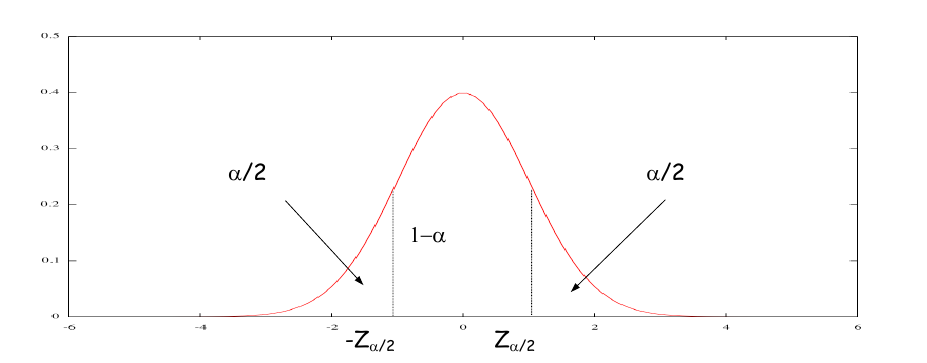
\includegraphics[width=.7\textwidth]{img/chapter-4/gaussain-confidence.png}
\caption{Intervallo di confidenza rispetto alla normale}\label{img:gaussian-confidence}
\end{figure}

Pertanto, essendo i valori della normale standard, noti, possiamo andare a scrivere la seguente probabilità:

\[
P(-z_{\alpha/2} \leq Z \leq z_{\alpha/2}) = 1 - \alpha
\]

Andando a sostituire con il valore che ci siamo calcolati a partire dalla variabile aleatoria associata alla distribuzione campionaria, si ha:
\[
P(-z_{\alpha/2} \leq \frac{\overline{X} - \mu}{\sigma/\sqrt{n}} \leq z_{\alpha/2}) = 1 - \alpha
\]

da cui:
\[
P\left (\overline{X} - z_{\alpha/2}\frac{\sigma}{\sqrt{n}} \leq \mu \leq \overline{X} + z_{\alpha/2}\frac{\sigma}{\sqrt{n}} \right ) = 1 - \alpha
\]
Da tale conclusione possiamo ricavare l'intervallo di confidenza (quindi i valori \(l\) e \(u\)).
Considerando quindi, \(\overline{x}\) la media della distribuzione campionaria, \(\sigma^2\) la varianza della popolazione iniziale (tale parametro non è banale) e sample size pari ad n, allora posso definire un \textbf{intervallo di confidenza} al \(100*(1-\alpha)\%\) di \textbf{livello di confidenza}, come: 

\[
\overline{x} - z_{\alpha/2}\frac{\sigma}{\sqrt{n}} \leq \mu \leq \overline{x} + z_{\alpha/2}\frac{\sigma}{\sqrt{n}}
\]
Con \(z_{\alpha/2}\) il punto di \(\frac{\alpha}{2}\)-quaritile o 100*(\(\frac{\alpha}{2}\))-percentile
\clearpage
Le considerazioni fatte sulla distribuzione iniziale